\section{Lezione 2016-10-24}
\subsection{TODO}
% Insert what you need. Any row is associated with the improvment or mistake
% arise. In the first column you can insert what you should resolve or change,
% instead in the second column you may put the section where to apply some
% modification.
\begin{table}[H]
\begin{center}
\begin{tabular}{|p{\textwidth}|c|}
\hline
\multicolumn{1}{|c|}{\textbf{Miglioramento}} & \textbf{Sezione} \\ \hline
\end{tabular}
\end{center}
\caption{Tabella miglioramenti}
\label{tab:tab_todo}
\end{table}

\subsection{Sul generatore di codice}
Il codice prodotto dal compilatore deve essere corretto, ovvero, deve
preservare la semantica (\textit{semantic preserving}) e dovrebbe essere di
alta qualit\'a. Ci\`o implica un uso efficacie delle risorse della macchina
obiettivo ed, attraverso una serie di euristiche, produrre un buon codice
vicono a quello ottimale (la produzione di codice ottimale \`e
\textbf{indicibile}).

\begin{figure}[H]
  \centering
  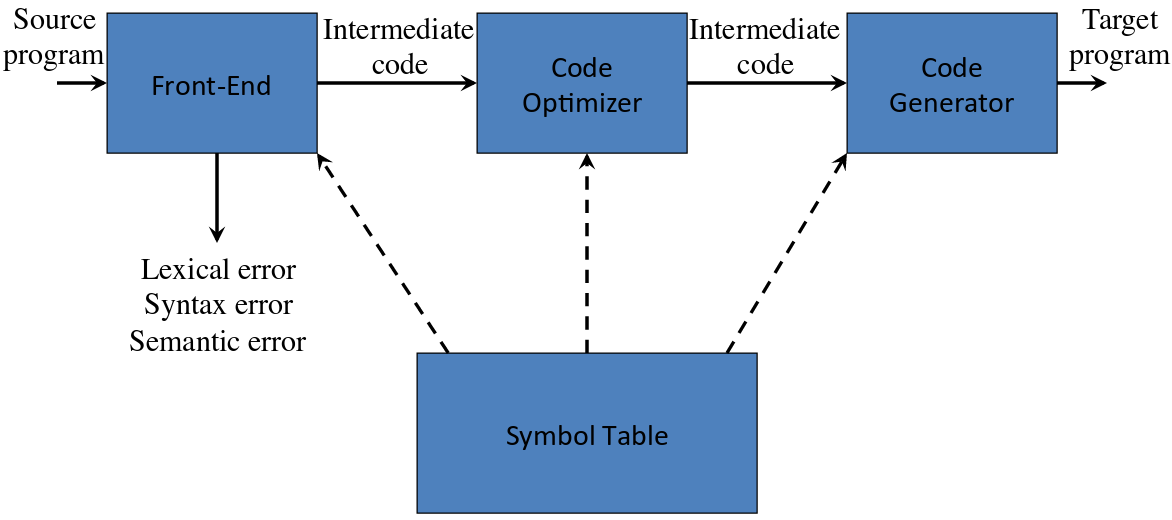
\includegraphics[scale=0.4]{res/image/code_generator_position}
  \caption{Posizione del generatori di codice}
  \label{img:code_generator_position}
\end{figure}

\subsection{Compiti del generatore}
Il \textit{code generator} ha tre compiti primari:
\begin{itemize}
\item selezione dell'istruzione
\item assegnazione ed allocazione dei registri
\item ordinamento delle istruzioni
\end{itemize}

Inoltre il compilatore pu\`o includere una fase di ottimizzazione (mappa l'IR
in input con IR ottimizzato) prima della generazione del codice.

\subsection{Variabili del generatore}
\subsubsection{L'input}
L'input del generatore \`e l'IR del codice sorgente, con i puntatori alle
informazioni salvate nella tabella dei simboli.
\subsubsection{Codice target}
Il \textit{backend} di un generatore di codice pu\`o generare differenze forme
di codice a seconda dei requisiti:
\begin{itemize}
\item codice macchina assoluto (codice eseguibile)
\item codice macchina riallocabile (file oggetto per il \textbf{linker})
\item linguaggio assembly (facilita il debuggin, ma richiede un assembly step)
\end{itemize}

\subsubsection{Architettura della macchina}
Definisce il set d'istruzioni avviabili, incluso il modello d'indirizzamento:
alto impatto sul codice generato.

Le macchine si vanno a dividire in due principali categorie:
\paragraph{CISC}
\begin{itemize}
\item istruzioni multi-clock
\item metodo d'indirizzamento complesso
\item serie di classi di registri
\item lunghezza variabile delle istruzioni in memoria
\end{itemize}
\paragraph{RISC}
\begin{itemize}
\item istruzioni single-clcok
\item molti registri
\item istruzioni a tre indirizzi
\item metodo d'indirizzamento semplice
\end{itemize}
\paragraph{Stack-based}
gli operandi sono inseriti nello stack e le operazioni sono eseguite nel top
(trattenute nei registri). In generale meno efficiente.

\subsection{Selezione dell'istruzione}
Uno comando pu\`o essere tradotto in vari modi. La scelta su quale set di
istruzioni convertirlo dipende da:
\begin{enumerate}
\item livello dell'IR
\item set d'istruzioni dell'architettura
\item la qualit\`a desiderata (es. efficienza) del codice generato
\end{enumerate}

\begin{figure}[H]
  \centering
  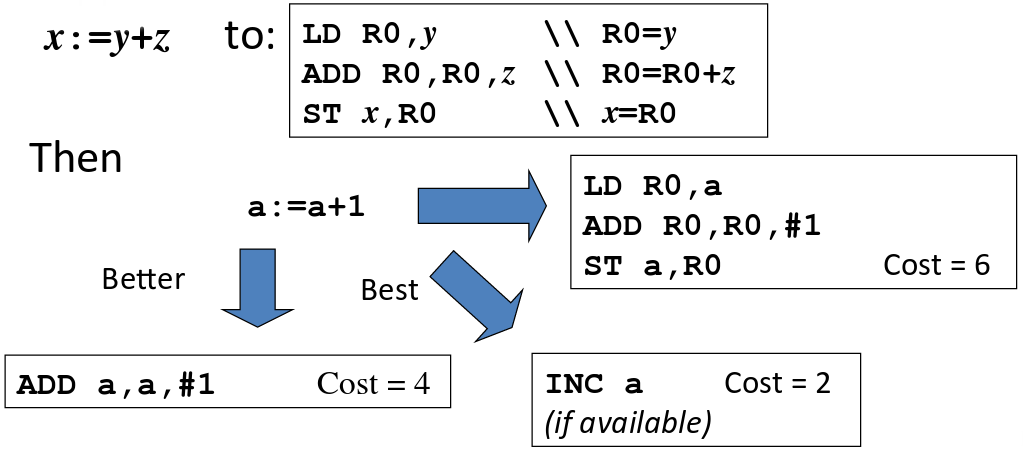
\includegraphics[scale=0.35]{res/image/choice_cost}
  \caption{Scelta del set di comandi in base al costo}
  \label{img:choice_cost}
\end{figure}

Per semplicit\`a dell'architettura possiamo definire il costo come
\begin{align*}
cost(\mathbf{OP \ dst}, \mathbf{src1}, \mathbf{src2})
&= 1 \\
&+ cost(dst\text{-}mode) \\
&+ cost(src1\text{-}mode) \\
&+ cost(src2\text{-}mode)
\end{align*}

La mappatura semplice delle singole istruzioni non garantisce una buona
qualit\`a del codice, in quanto non si va ad osservarlo nella usa interezza.

\begin{figure}[H]
  \centering
  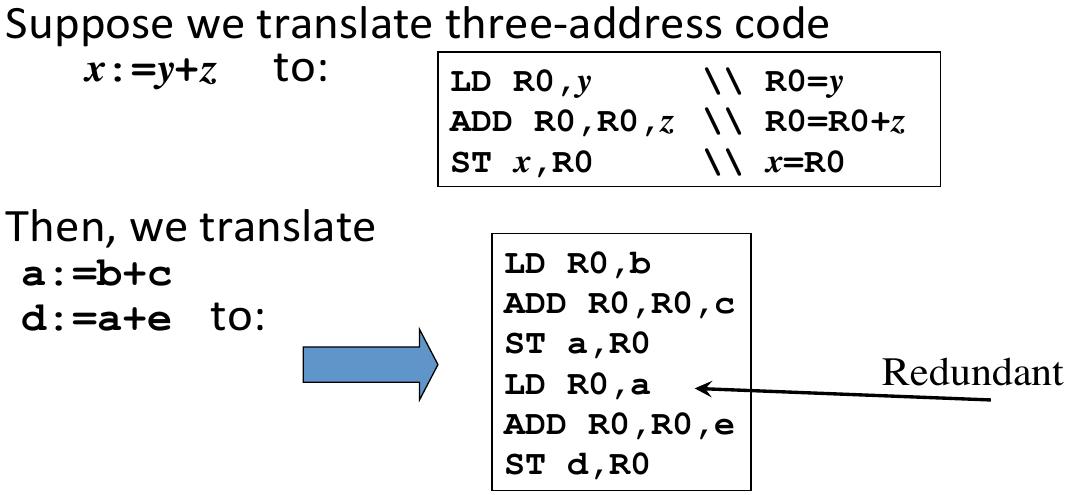
\includegraphics[scale=0.35]{res/image/needed_global_optimization}
  \caption{Necessarie ottimizzazione globali per eliminare ridondanze}
  \label{img:needed_global_optimization}
\end{figure}

Si possono fare due accorgimenti per garantire una buona qualit\`a del codice:
\paragraph{Allocazione ed assegnazione dei registri}
L'uso efficiente di un piccolo insieme di registri \`e importante per generare
buon codice. I registri sono assegnati per:
\begin{itemize}
\item \textit{Register Allocation} - per selezionare l'insieme delle variabili
che risiederanno nei registri a quel punto del codice
\item \textit{Register Assignment} - per scegliere in quale registro la
variabile risiedera
\end{itemize}
Trovare un insieme di registri ottimali \`e un problema in
\textit{NP-completo}.
\paragraph{Scelta dell'ordine di istruzioni}
L'ordine delle istruzioni potrebbe portare ad un miglioramento delle
prestazioni del programma. Se le istruzioni sono indipendenti, l'ordine di
valutazione pu\'o cambiare.

\begin{figure}[H]
  \centering
  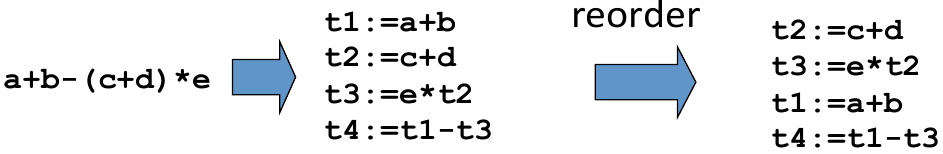
\includegraphics[scale=0.5]{res/image/reorder_variable}
  \caption{Riordinamento di variabili indipendenti}
  \label{img:reorder_variable}
\end{figure}

\subsection{Towards Flow Graphs}
